% IEEE RT 2026 supporting document (max 2 pages target)
% Free format; can include figures.

\documentclass[10pt]{article}
\usepackage[margin=0.75in]{geometry}
\usepackage[T1]{fontenc}
\usepackage[utf8]{inputenc}
\usepackage{graphicx}
\usepackage{amsmath}
\usepackage{booktabs}
\usepackage{hyperref}
\usepackage{multicol}
\usepackage{subcaption}
\usepackage{amssymb}
\hypersetup{colorlinks=true,linkcolor=blue,urlcolor=blue,citecolor=blue}

\begin{document}

\begin{center}
{\Large \textbf{Design-Space Exploration and Integer Quantization of Graph Neural Networks for Real-Time FPGA Track Finding}}\\
\vspace{0.2em}
{Pelayo Leguina}\\
\vspace{0.2em}
{\small IEEE Real-Time 2026 (25--29 May 2026), La Biodola -- Isola d'Elba, Italy}
\end{center}

\vspace{-0.3em}
\section*{Motivation and Context}
Fixed-latency trigger/DAQ systems in the CMS Level-1 upgrade (12.5~$\mu$s budget~\cite{CMS_PHASE2_TDR}) demand inference architectures that balance accuracy with hardware feasibility under strict throughput and resource constraints. Displaced-muon signatures from long-lived particles pose unique challenges for traditional pattern-based track finding because they deviate from prompt-track assumptions. Graph neural networks (GNNs) naturally represent sparse, irregular detector geometries: nodes encode stub-level features and edges capture local geometric compatibility, making them well-suited for the overlap muon track finder region~\cite{OMTF_JINST} where barrel and endcap detectors meet.

\vspace{-0.2em}
\section*{Methodology and Workflow}
This work develops a reproducible pipeline from PyTorch Geometric model training to FPGA-ready HLS implementations. Unlike automated ML toolflows that primarily target dense or convolutional layers, message-passing GNN operations require explicit handling of irregular aggregation patterns, dynamic data movement, and careful numeric design. Our framework includes: (i) multiple HLS implementation paths (floating-point baseline, PTQ-Float hybrid, and pure integer PTQ-INT8); (ii) automated design-space exploration (DSE) across architectural, quantization, and microarchitectural parameters; (iii) data-driven bit-width optimization for minimizing resource usage while maintaining numerical correctness.

\vspace{-0.2em}
\section*{Model Training and Quantization}
GraphSAGE architecture: feature projection (1433$\to$16), two message-passing layers (16$\to$24$\to$7). \emph{Base model} (Cora, 1000 nodes): 80.3\% accuracy. \emph{Reduced variant} (24K parameters, FPGA-compatible): 75.8\% accuracy. \emph{Post-training quantization (PTQ)} to INT8 maintains 75.7\% accuracy (0.1\% degradation). \emph{Quantization-aware training (QAT)} is under active development; preliminary experiments show 28.2\% accuracy, indicating the current 16$\times$24 architecture has insufficient capacity for QAT—larger models (32$\times$48) are being explored. See Table~1.

\vspace{-0.2em}
\section*{Integer-Only Implementation and Validation}
PTQ-INT8 datapath: INT8 weights/activations, INT32 biases, INT16 adjacency ($K=2^{12}$). Fixed-point scaling: $y = \mathrm{clamp}\big((a\cdot s_{\text{fp}} + 2^{M-1}) \gg M\big)$. \emph{HLS C-simulation validation}: M=24 achieves \textbf{0~LSB error} vs Python integer emulator on 8-node subgraphs; M=20 yields $\leq$13~LSB with narrower multipliers. Data-driven bit-width optimization analyzes actual ranges to reduce accumulator/scaling widths (22/21/43 bits vs 32/32/64 conservative defaults), saving 42 bits in critical paths.

\vspace{-0.2em}
\begin{table}[h!]
\centering
\small
\begin{tabular}{lcccc}
\toprule
Model Variant & Test Accuracy & Parameters & Memory & Status\\
\midrule
Base (float) & 80.3\% & 184K & 0.70~MB & Complete\\
Reduced (float) & 75.8\% & 24K & 0.09~MB & Complete\\
PTQ-INT8 & 75.7\% & 24K & 0.02~MB & HLS C-sim validated\\
QAT-INT8 (16$\times$24) & 28.2\% & 24K & 0.02~MB & In progress\\
\bottomrule
\end{tabular}
\vspace{-0.2em}
\caption{Model accuracy on Cora dataset. PTQ preserves accuracy; QAT under development with larger architectures.}
\label{tab:results}
\vspace{-0.8em}
\end{table}

\vspace{-0.2em}
\section*{Design Space Exploration Framework}
The DSE framework is designed to explore: (i) \emph{algorithm level}—hidden dimensions (16-32), fixed-point precision $M$ (20-28 bits); (ii) \emph{quantization level}—unroll factors, accumulator bit-widths; (iii) \emph{HLS level}—pipeline initiation intervals, resource binding. Each design point executes the full automated flow: PTQ parameter generation → test vector creation → HLS synthesis → report parsing. Pareto analysis will identify non-dominated solutions across accuracy, latency, and resource usage (Fig.~\ref{fig:results})~\cite{Hamilton2017}. Initial validation demonstrates the methodology on a baseline design point; comprehensive sweeps are in progress.

\vspace{-0.3em}
\begin{figure}[h!]
\centering
\begin{subfigure}{0.48\textwidth}
  \centering
  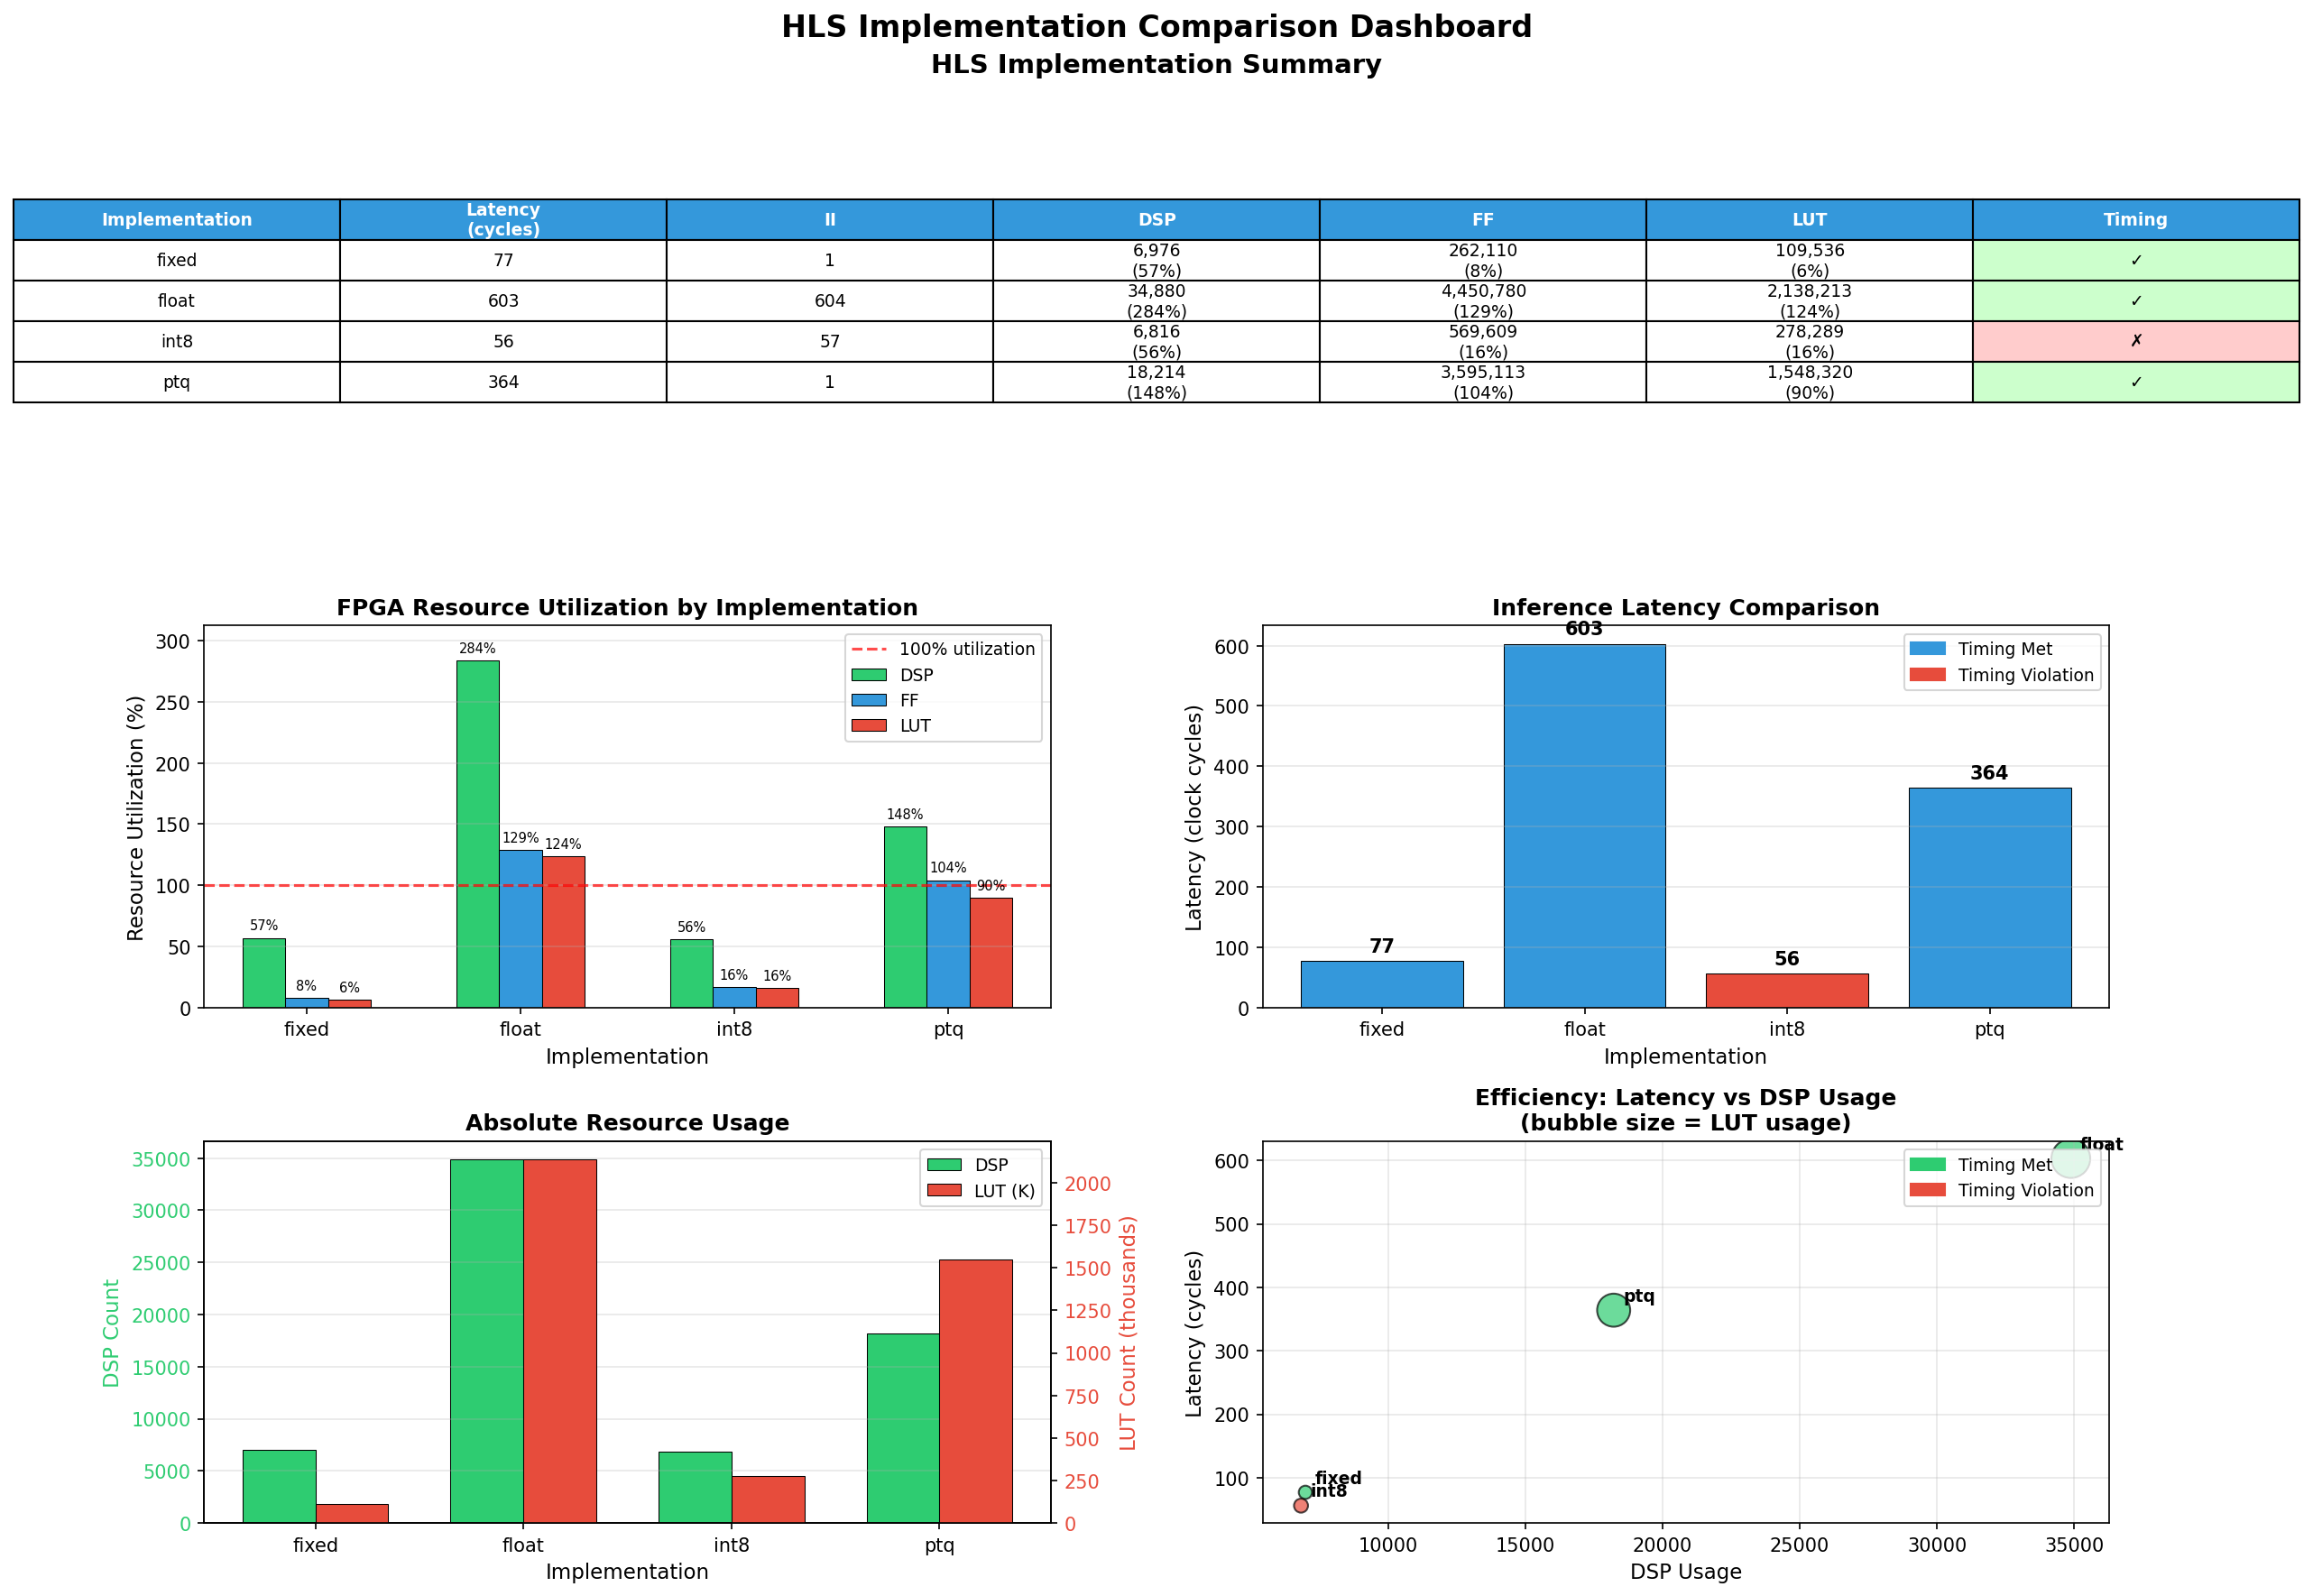
\includegraphics[width=\textwidth]{figures/hls_comparison.png}
  \caption{Preliminary HLS synthesis results showing float vs PTQ-INT8 comparison on Xilinx VU13P.}
\end{subfigure}
\hfill
\begin{subfigure}{0.48\textwidth}
  \centering
  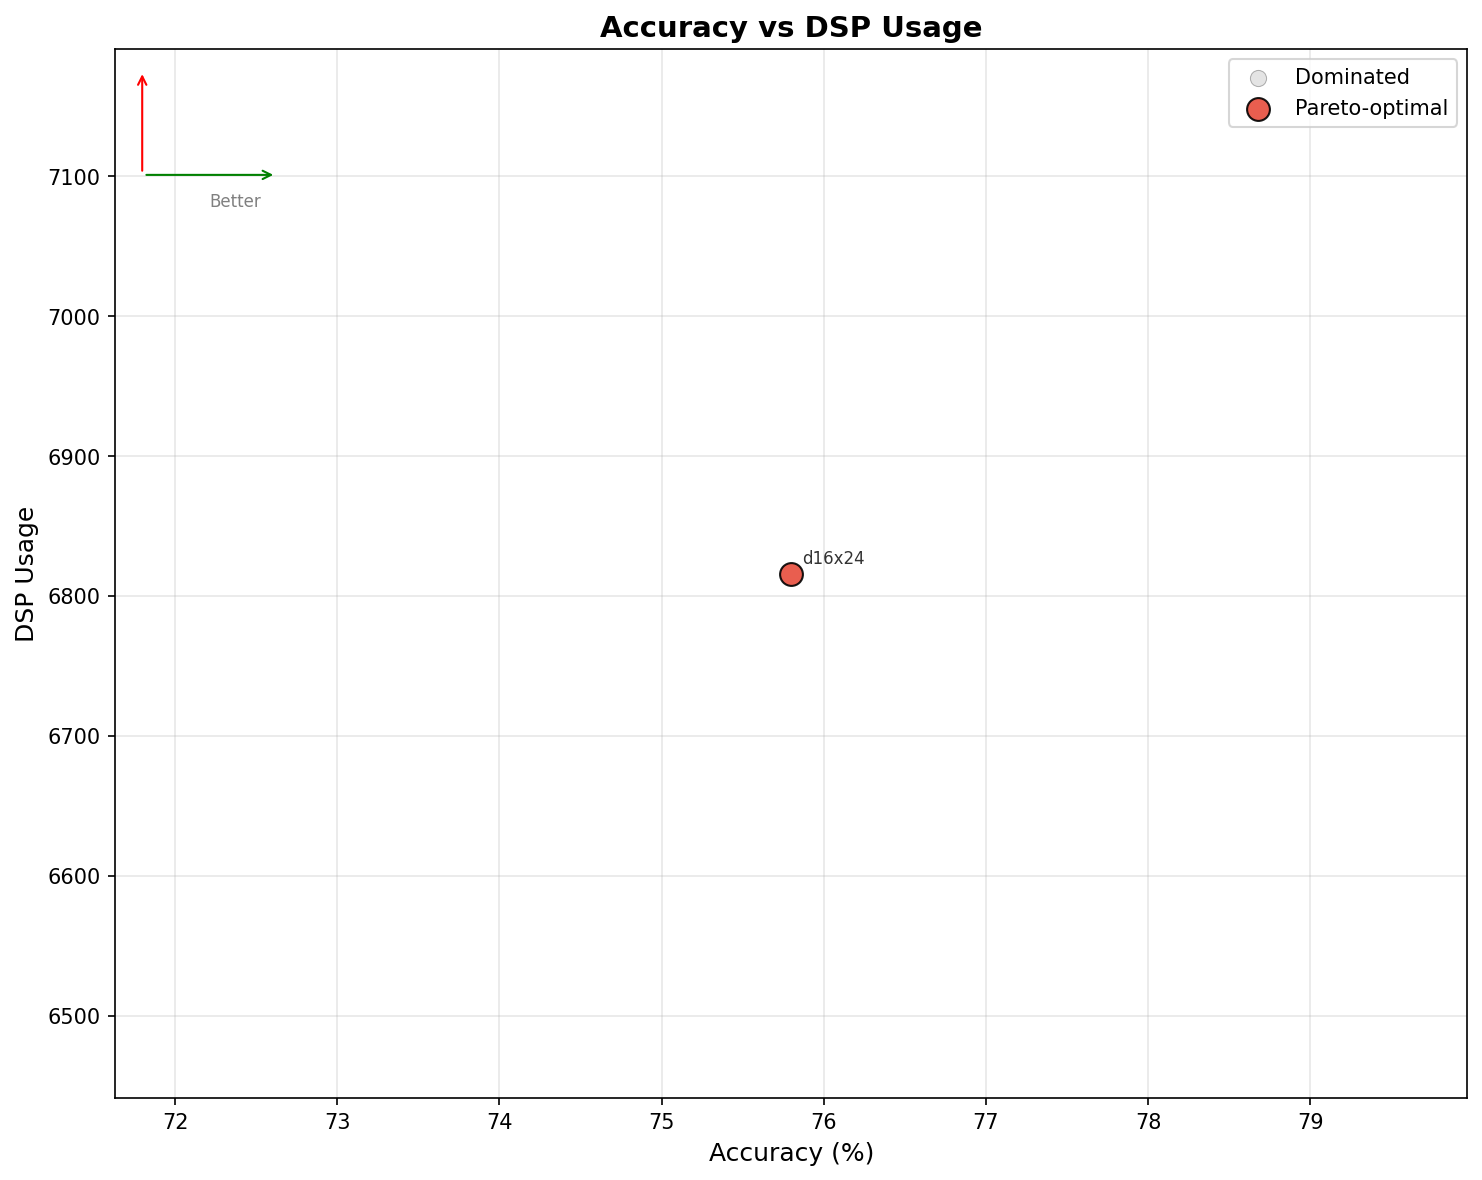
\includegraphics[width=\textwidth]{figures/pareto_accuracy_vs_dsp_used.png}
  \caption{DSE Pareto framework (initial baseline point shown; full sweep in progress).}
\end{subfigure}
\vspace{-0.2em}
\caption{Preliminary results and DSE framework. Full design space exploration is ongoing.}
\label{fig:results}
\vspace{-0.6em}
\end{figure}

\vspace{-0.2em}
\section*{Current Status and Next Steps}
\emph{Completed}: Model training, PTQ-INT8 implementation, HLS C-simulation validation (0~LSB error), automated DSE infrastructure, bit-width optimization tools. \emph{In progress}: QAT with larger architectures, comprehensive DSE parameter sweeps, displaced-muon dataset integration, track-finder graph definition (nodes=DT/CSC/RPC stubs~\cite{OMTF_JINST}, edges=$\Delta\eta$-$\Delta\phi$ geometric constraints). \emph{Planned}: Retrain on physics data, optimize for 12.5~$\mu$s latency~\cite{CMS_PHASE2_TDR}, deploy on Phase-2 FPGAs.

\vspace{-0.2em}
\section*{Reproducibility}
Full workflow automation: \texttt{run\_pipeline.py} (main pipeline), \texttt{explore\_design\_space.py} (DSE orchestration), \texttt{hls/} (HLS kernels). Configuration: \texttt{model\_config.yaml}, \texttt{design\_space.yaml}. Verification: \texttt{tests/} validate bit-exact Python-HLS agreement at each pipeline stage.

\vspace{-0.2em}
\section*{References}

\begin{thebibliography}{9}

\bibitem{Hamilton2017}
W.~L. Hamilton, R.~Ying, and J.~Leskovec,
``Inductive Representation Learning on Large Graphs,''
\emph{arXiv:1706.02216} (2017), \url{https://arxiv.org/abs/1706.02216}.

\bibitem{CMS_PHASE2_TDR}
CMS Collaboration, \textit{The Phase-2 Upgrade of the CMS Level-1 Trigger}, CERN-LHCC-2020-004, CMS-TDR-021, Geneva (2020), \url{https://cds.cern.ch/record/2714892}.

\bibitem{OMTF_JINST}
K. Bunkowski et al., \textit{The Overlap Muon Track Finder of the CMS experiment}, JINST \textbf{11}, C03004 (2016), \url{https://doi.org/10.1088/1748-0221/11/03/C03004}.

\bibitem{CMS_TRIGGER}
CMS Collaboration, \textit{The CMS trigger system}, JINST \textbf{12} (2017) P01020, \url{https://doi.org/10.1088/1748-0221/12/01/P01020}.

\end{thebibliography}

\end{document}
